\documentclass [a4paper,10pt] {article}
\usepackage[latin1]{inputenc}
\usepackage[ngerman]{babel}
\usepackage[T1]{fontenc}
\usepackage{amsmath, amsthm, amssymb}
\usepackage{latexsym}
\usepackage{graphicx}
\usepackage{a4wide}
\setlength{\parindent}{0mm}
\setlength{\parskip}{3mm}
\usepackage{fancyhdr}
\renewcommand{\labelenumi}{(\alph{enumi})}
\pagestyle{fancy}
\headheight 16pt
\renewcommand{\headrulewidth}{0.4pt}
\renewcommand{\footrulewidth}{0.4pt}
\renewcommand{\familydefault}{\sfdefault}
\lhead{Lego Mindstorms Praktikum}
\chead{Team A}
\rhead{SS 2010}
\begin{document}
%\pagestyle{empty}%
%\tableofcontents %
%\newpage%

%content ab hier
%\begin{description}
%	\item[] \emph{} $\rightarrow$ 
%	\includegraphics[width=10cm]{}
% \end{description} 

\section{Vor�berlegungen}
\subsection{Aufgabenstellung}
Es sind Robotor zu konstruieren, die ein Sokoban-Spiel zun�chst einlesen und dann l�sen. Zu den Regeln eines normalen Sokoban--Spiels wird hierbei zus�tzlich zu dem Schieber ein Zieher eingesetzt. Au�erdem wird ein Kartierer ben�tigt und ein Bauteil, dass die L�sung des Spiels berechnet. \\
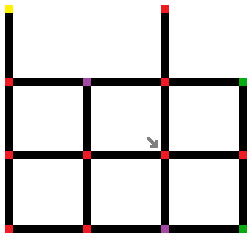
\includegraphics[width=10cm]{soko.png} \\
Das Feld besteht aus schwarzen Linien. Die Kreuzungen sind durch verschiedene Faben gekennzeichnet. Gr�n steht f�r die Ziele der Kisten, Violett f�r die Startr�ume, Gelb f�r den Startraum des Schiebers und ein Pfeil markiert den Startraum des Ziehers und des Kartierers. Rot wird f�r normale Kreuzungen verwendet. 
\subsection{Zeitplan}
	\textbf{Beginn:} 10. September 2010 \\
	\textbf{Abgabe:} 27. September 2010
	
	\textbf{Konstruktion der Roboter:} ca. 1 Tag \\
	\textbf{Testen von Sensoren und anderen Komponenten:} ca. 2 Tage \\
	\textbf{Implementierung der zusammenfassenden Navigation:} ca. 2 Tage \\
	\textbf{Implementierung des Kartierers:} ca. 3-4 Tage \\
	\textbf{Implementierung des Planers:} ca. 4-5 Tage \\
	\textbf{Implementierung des Ziehers:} ca. 3 Tage \\
	\textbf{Implementierung des Schiebers:} ca. 3 Tage \\
	\textbf{Testen und Optimierung:} ca. 3-4 Tage	
\subsection{Aufgabenverteilung}
	\textbf{Teammitglieder:} \\
Andreas Bigontina, Michael Bigontina,  Christoph Bruns,  Maximilian Burger, Sebastian Hagen, Wiebke K�pp,Anastasia Panteloglou, Till Rohrmann 

	\textbf{Organisation:} \\ 
Till Rohrmann, Wiebke K�pp \\
	\textbf{Kartierer:} \\ 
Maximilian Burger, Sebastian Hagen \\
	\textbf{Planer:} \\
Till Rohrmann\\ 
	\textbf{Zieher:} \\
Christoph Bruns, Michael Bigontina \\	
	\textbf{Schieber} \\ 
Andreas Bigontina, Anastasia Panteloglou \\
	\textbf{Fehlerbehandlung:} \\
Wiebke K�pp	
\subsection{L�sungsansatz}
	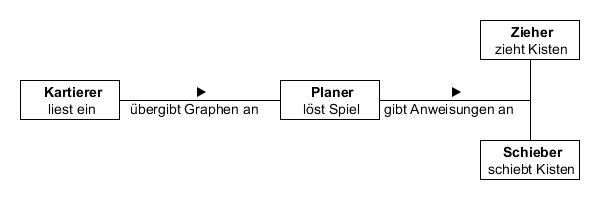
\includegraphics[width=13cm]{sol.jpg} \\
	\textbf{Navigation:} \\
	Alle drei Roboter sollen eine gemeinsame Navigation verwenden. Die Roboter sollen mit dieser durch einfache Befehle wie \emph{'Bewege dich nach Norden'} oder \emph{'Bewege dich zum n�chsten Raum'} gesteuert werden. Au�erdem sollen auch Koordinaten angegeben werden k�nnen zu denen sich ein Roboter bewegen soll. \\
	Die Navigation wird mithilfe eines Pilot realisiert, der �ber verschiedene Behaviors sicherstellt, dass die Roboter der Linie folgen und von ihr nicht abweichen und das R�ume erkannt werden.
	
	\textbf{Kartierer:} \\
Der Kartierer beginnt an seinem Startpunkt das Feld einzulesen. Er speichert das Feld in einem Graphen, in dessen Knoten Informationen �ber den Typ des jeweiligen Knotens (definiert durch die Farbe) und dessen Nachbarn (im Norden, Osten, S�den und Wesen) gespeichert sind. Der Startpunkt ist hierbei als Punkt (0,0) definiert. Die Ausrichtung zu Beginn wird als Norden definiert. Bewegt sich der Roboter nun nach Norden wird die y--Koordinate inkrementiert, bei Osten wird die x--Koordinate inkrementiert und bei S�den und Westen werden x- und y--Koordinate dekrementiert. \\
Der Kartierer f�hrt nun eine Tiefensuche auf dem Feld aus und analysiert jede Kreuzung, die er zuvor noch nicht analysiert hat, indem er sich auf ihr dreht und die Richtungen speichert, die dieser Knoten besitzt. \\
Nach dem kartieren schickt der Roboter den gesamten Graphen per Bluetooth an den Computer, der dann die Berechnung der L�sung durchf�hrt.
	
	\textbf{Planer:} 
Da die Leistung eines Bricks vorraussichtlich nicht f�r die Berechnung der L�sung ausreicht, wird die Berechnung auf einem Computer durchgef�hrt. 

	\textbf{Schieber:}


	\textbf{Zieher:}



\end{document}